In this chapter we describe a collection of novice interactions with the
\ocaml compiler --- including, importantly, type errors --- that we
gathered at UC San Diego over two quarters of the undergraduate CSE 130
course (IRB \#140608).
%
We have made the anonymized data publicly
available~\citep{Seidel2017-ko}, and hope that other researchers will
find it as valuable as we have.

The CSE 130 course is an upper-level (\ie generally consisting of third-
and fourth-year students) course that introduces students to typed
functional languages, specifically \ocaml.
%
For most students, this course will be their first exposure to both
functional programming and type systems with global inference.
%
We generally spend the first five weeks covering basic functional
programming in \ocaml, and then spend the last five weeks in
\textsc{Scala} covering more advanced concepts like traits and
monads (in the guise of |for-yield| comprehensions).
%
In the \ocaml portion of the course we cover standard functional idioms
like (tail-) recursion, higher-order functions, and user-defined
algebraic datatypes.

We recruited students from two instances of the course, Spring 2014
(\SPRING) and Fall 2015 (\FALL), to use an instrumented version of the
\ocamltop\footnote{\url{https://www.typerex.org/ocaml-top.html}} editor, which logged each of their
interactions with the \ocaml top-level system.
%
46 students from the \SPRING quarter and 56 students from the \FALL
quarter participated, for a total of 102 participants.
%
The participants used our instrumented editor to complete the first
three programming assignments, which involved writing 23 \ocaml
programs.
%

\begin{figure}
\centering
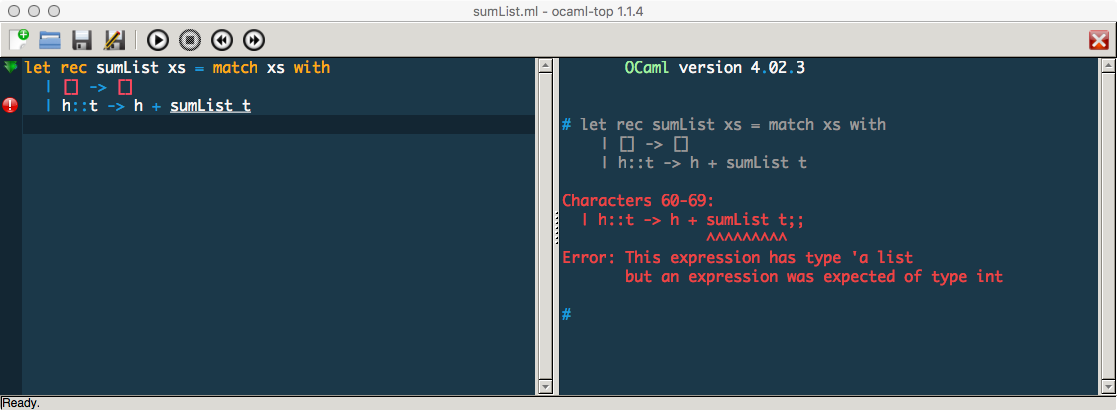
\includegraphics[width=\linewidth]{ocaml-top.png}
\caption{The \ocamltop editor. \ES{TODO: figure out how to cite}}
\label{fig:intro:ocaml-top}
\end{figure}

\autoref{fig:intro:ocaml-top} shows the main interface of \ocamltop,
which contains an editor pane on the left and an instance of the \ocaml
top-level interpreter on the right.
%
The students interact with the top-level system by selecting text in the
editor and pressing the ``play'' button in the toolbar, which sends the
selected text to the interpreter for evaluation.
%
The editor also maintains a cursor into the open file to track how much
of the file has been evaluated; this allows it to intelligently send the
next top-level definition to the interpreter if no text is selected.
%
The toolbar also has a ``stop'' button to abort evaluation (\eg to abort
infinite loops), a ``rewind'' button to restart the interpreter, and a
``fast-forward'' button to load the entire file into the interpreter.
%
\ocamltop always sends each definition to the interpreter individually,
even when using the ``fast-forward'' button, this will become important
when we extract ill-typed programs from the interaction traces.

We instrumented \ocamltop to record each of the student's interactions
with the top-level interpreter.
%
Specifically, we modified it to log an event each time a student pressed
one of the four interaction buttons on the toolbar (or used the
equivalent keyboard shortcuts).
%
This gives rise to three kinds of interaction events:
%
\begin{description}
\item[\textsc{Eval}] The student sent one or more definitions to be
  evaluated by the interpreter, by pressing either ``play'' or
  ``fast-forward''. In addition to logging the event, we logged both the
  offsets into the file that mark the region of text that was evaluated,
  and the list of top-level definitions that were evaluated.
\item[\textsc{Abort}] The student aborted evaluation by pressing
  ``stop''.
\item[\textsc{Stop}] The student restarted the interpreter by pressing
  ``rewind''.
\end{description}
%
For each event we also recorded the filename to identify the homework
the student was working on, the current UNIX timestamp, the entire body
of the file, and the offset of the cursor into the file.
%
Thus, for each participating student we can see and replay, with fine
granularity, the steps they took to solve the programming assignments.

We then post-processed the interaction traces to add the \ocaml
interpreter's responses to the students' submissions.
%
Recall that \ocamltop always sends single top-level definitions to the
interpreter, which maintains an environment of defined types and
functions.
%
This is inconvenient for extracting ill-typed programs, as the vast
majority of submitted definitions will depend on other definitions
that were submitted previously.
%
Thus, we modified the \ocaml interpreter to track dependencies between
top-level function and type definitions, so that for each definition a
student submitted, we could produce a self-contained, \emph{minimal}
program that would have the same behavior.

For each submitted definition, we collected the interpreter's response
and the minimal self-contained program, and classified the response as
either a syntax error, a scoping error (\eg an unbound variable), a type
error, or no error.
%
As we are primarily concerned with type errors in this work, we did not
capture the actual result of evaluating the definition, \ie the
resulting value, but it would be easy to extend the replay procedure to
do so.
%
We then stored the post-processed interaction traces as sequences of
JSON objects, in the format described by
\autoref{fig:intro:data-format}.
%
\begin{figure}
\centering
\begin{lstlisting}
{
    "file": "hw1.ml" | "hw2.ml" | "hw3.ml",
    "time": number,
    "body": string,
    "cursor": number,
    "event": {
        "type": "abort" | "eval" | "stop",
        "region": {
            "start": number,
            "stop": number
        }
    },
    "ocaml": [{
        "in": string,
        "out": string,
        "type": "scope" | "syntax" | "type" | "",
        "min": string
    }]
}
\end{lstlisting}
\caption{Format of the post-processed interaction events as JSON
  objects.}
\label{fig:intro:data-format}
\end{figure}
%
From this format it is quite convenient to run various analyses, \eg
what are the hardest assignments (measured by time spent or by errors
encountered), what is the relative frequency of various errors, \etc,
though for this work we will only use the dataset as a source of type
errors and fixes.

%% TODO: weird, this doesnt seem to be a problem anymore??
% In retrospect, it is not clear that the evaluation model used by
% \ocamltop, \ie loading individual definitions rather than the entire
% file, is the best model for students learning the language.
% %
% This model can lead to very subtle issues where the state of the program
% as represented by the file (and, presumably, the state according to the
% student's mind) diverges from the state of the interpreter.
% %
% Consider the following, suppose the student defines her own type for
% lists of integers and then defines a simple function to sum the integers
% of a list.
% %
% \begin{code}
%   type intlist = Nil | Cons of int * intlist

%   let rec sum xs = match xs with
%     | Nil         -> 0
%     | Cons (h, t) -> h + sum t
% \end{code}
% %
% The \ocaml interpreter will accept her definitions, having inferred that
% |sum| must have type |intlist -> int|.
% %
% But suppose now she decides to make |intlist| polymorphic in the
% element, changing the |intlist| definition to
% %
% \begin{code}
%   type 'a intlist = Nil | Cons of 'a * 'a intlist
% \end{code}
% %
% Then she tries to call the |sum| function.
% %
